\documentclass[11pt, oneside]{article}   	% use "amsart" instead of "article" for AMSLaTeX format
\usepackage{geometry}                		% See geometry.pdf to learn the layout options. There are lots.
\geometry{letterpaper}                   		% ... or a4paper or a5paper or ... 
%\geometry{landscape}                		% Activate for for rotated page geometry
%\usepackage[parfill]{parskip}    		% Activate to begin paragraphs with an empty line rather than an indent
\usepackage{graphicx}				% Use pdf, png, jpg, or eps� with pdflatex; use eps in DVI mode
								% TeX will automatically convert eps --> pdf in pdflatex		
\usepackage{amssymb}
\usepackage{amsmath}
\usepackage{parskip}

\title{Integrating cosine squared}
%\author{The Author}
%\section{}
% \subsection*{R code}
\date{}							% Activate to display a given date or no date

\graphicspath{{/Users/telliott_admin/Dropbox/Tex/png/}}

% \begin{lstlisting}  \end{lstlisting}
% \begin{center} 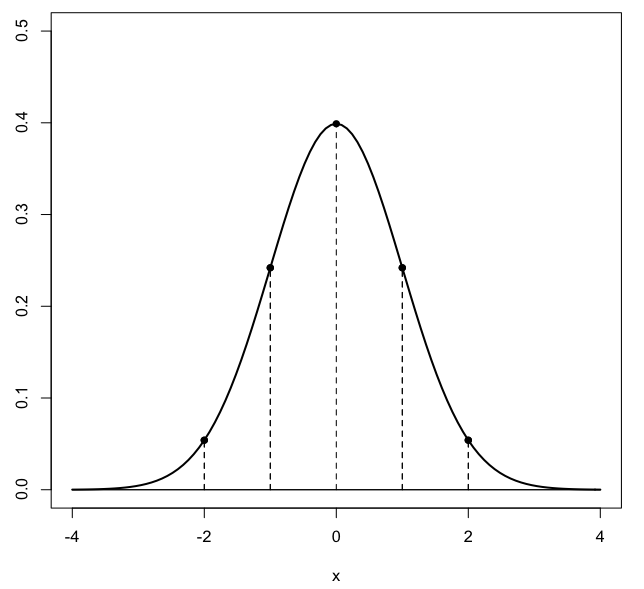
\includegraphics [scale=0.4] {gauss3.png} \end{center}
% \begin{bmatrix} a  &  b \\ c  &  d \end{bmatrix}
% \bigg |_

\begin{document}
\maketitle
\noindent
\Large

We want to find the integral of
\[ \int \cos^2 x \ dx \]

It's a very common integral in problems with trig substitution and otherwise.  The first thing to note is that 
\[ \int \sin^2 x \ dx \]

is the same problem, because
\[ \sin^2 x + \cos^2 x = 1 \]

so 
\[ \int \sin^2 x \ dx + \int \cos^2 x  \ dx = \int 1 \ dx = x \]

\subsection*{method 0}
I call this method 0 because it's not really methodical.  The first approach is to guess.  If you play around differentiating products of functions (like $e^x$, $\ln x$, $\sin x$, $\cos x$ and $x$), you will discover that
\[ \frac{d}{dx} \ [ \ \sin x \cos x \ ] \ = -\sin^2 x + \cos^2 x \]
\[ = \cos^2 x - 1 +  \cos^2 x \]
\[ = 2 \cos^2 x - 1 \]

Integrating both sides, we obtain
\[ \sin x \cos x = 2 \int \cos^2 x \ dx - x \]

and rearranging:
\[ \int \cos^2 x \ dx = \frac{1}{2} (x + \sin x \cos x) \]

\subsection*{method 1}
There are two other systematic approaches that can be contrasted.  The first, which is arguably the simpler one, is to remember the addition formula for cosine
\[ \cos (s+t) = \cos s \cos t - \sin s \sin t \]

The trick I use to remember these formulas is to work out the consequences for this one:
\[ \cos (s-t) = \cos s \cos t + \sin s \sin t \]

This makes perfect sense since if $s=t$ then we get
\[ \cos 0 = \cos^2 s + \sin^2 s = 1 \]

which we know is correct.  So
\[ \cos (s+t) = \cos s \cos t - \sin s \sin t \]

If $s=t$ then (changing to $x$)
\[ \cos 2x = \cos^2 x  - \sin^2 x \]

and using the standard identity $\cos^2 x + \sin^2 x = 1$ this becomes
\[ \cos 2x = 2\cos^2 x - 1 \]

The "double angle" formula.

\[ 2 \cos^2 x = 1 + \cos 2 x \]
\[ \cos^2 x= \frac{1}{2} ( 1 + \cos 2x )  \]
Integrating
\[ \int \cos^2 x \ dx = \int \frac{1}{2} ( 1 + \cos 2x ) \ dx \]
\[ \frac{1}{2} ( x + \frac{1}{2} \sin 2x ) \]
We check by differentiating.  Leaving the factor of $1/2$ out, we obtain for $d/dx$:
\[ 1 + \cos 2x \]
which, as we saw above, is equal to $2 \cos^2 x$.  Remembering the factor of $1/2$, we obtain the expected result.

Comparing our results so far, we have obtained different answers, namely
\[ \int \cos^2 x \ dx = \frac{1}{2} (x + \sin x \cos x) \]

\[ \int \cos^2 x \ dx = \frac{1}{2} ( x + \frac{1}{2} \sin 2x ) \]

which indicates (if there is no mistake), that
\[ \sin x \cos x = \frac{1}{2} \sin 2x  \]

to see that this is correct, recall the addition formula for sine:
\[ \sin (s+t) = \sin s \cos t + \sin t \cos s \]

then if $s=t$
\[ \sin 2s = 2 \sin s \cos s  \]

with a slight rearrangement, this is indeed what we had.

\subsection*{method 2}
In the second "method", we do a substitution to take advantage of the integration by parts formula

\[ \int u \ dv = uv - \int v \ du \]
Let $u=\cos x$, then $du = -\sin x \ dx$, and let $dv = \cos x \ dx$ then $v= \sin x$, so
\[ \int \cos^2 x \ dx = \sin x \cos x + \int \sin^2 x \ dx \]

This still seems like not much progress since (as we saw) $\int \sin^2 x \ dx$ is really the same problem as $\int \cos^2 x \ dx$
\[ \int \sin^2 x \ dx = \int (1 - \cos^2 x) dx = \int dx - \int \cos^2 x dx \]

but, forging ahead
\[ \int \cos^2 x \ dx = \sin x \cos x + \int \sin^2 x \ dx \]
\[ \int \cos^2 x \ dx = \sin x \cos x  + x -  \int \cos^2 x dx \]

Rearranging:
\[ \int \cos^2 x \ dx  = \frac{1}{2} \ [ \ \sin x \cos x + x \ ] \ \]

which is what we had before.

\subsection*{Dealing with higher powers}
Most higher powers of sine and cosine are fairly easy to work with, after using the basic trig identity.  Here is the cube:
\[ \int \cos^3 x \ dx = \int (1 - \sin^2 x) \cos x \ dx \]

We end up with two terms, $\int \cos x \ dx$, which is trivial, and $\int \sin^2 x \cos x \ dx$, which yields to substitution (let $u = \sin x$).

But, sometimes, we get an even power, for example:

\[ \int \cos^4 x \ dx \]

What this problem needs is to forget about the integration for a moment and do two applications of the double angle formula:
\[ \cos^2 x= \frac{1}{2} ( 1 + \cos 2x )  \]

Rewrite
\[ \cos^4 x = (\cos^2 x)^2 \]
\[ = \ [ \ \frac{1}{2} ( 1 + \cos 2x ) \ ]^2 \]
\[ = \frac{1}{4}(1 + 2 \cos 2x + \cos^2 2x) \]

now use the formula a second time to substitute for 
\[ \cos^2 2x = \frac{1}{2} ( 1 + \cos 4x )  \]

I get 
\[ \cos^4 x = \frac{3}{8} + \frac{1}{2} \cos 2x + \frac{1}{8} \cos 4x \]
\[ \int \cos^4 x \ dx = \frac{1}{8} \int \ [ \  3 + 4 \cos 2x + \cos 4x \ ] \ dx \]
\[ = \frac{1}{8} \ [ \ 3x + 2 \sin 2 x + \frac{1}{4} \sin 4x \ ] \]

See Strang (pp 289-290).

\end{document}  